\begin{table}[!htb]
  \caption{\textit{Continuação} - Práticas identificadas no pensamento computacional, segundo \citeonline{Barr2011}, presentes/possíveis na educação básica}
  \label{tab:facetas}
  \begin{center}
    \begin{tabularx}{\textwidth}{@{}YYYYYY@{}}
      \hline 
      
      \textbf{Práticas} & \textbf{Matemática} & \textbf{Ciências} & \textbf{Estudos Sociais} & \textbf{Linguagens} \\

      \hline
      \\
      \textit{Procedimentos algorítmicos} & Longa divisão, fatoração & Fazer procedimentos experimentais & - & Escrever instruções \\ \\ % 

      \hline
      \\
      \textit{Automação} & - & Usar \textit{Probware} ou \textit{Origin} & Usar excel & Usar um corretor ortográfico \\ \\ 

      \hline
      \\
      \textit{Paralelização} & Resolver sistema lineares; fazer multiplicação de matrizes & Executar simultaneamente experimentos com diferentes parâmetros & - & - \\ \\

      \hline
      \\
      \textit{Simulação} & Representar graficamente uma função em um plano cartesiano e modificar os valores da variáveis & Simular o movimento de o sistema solar & Jogar Age of Empires; Trilha de Oregon & Fazer uma reencenação de uma história \\ \\
      \hline

    \end{tabularx}
  \end{center}
  \legend{Fonte: Adaptado de \citeonline{Barr2011}}
\end{table}

\begin{table}[htbp]
  %  \centering does nothing if table is full width
    \caption{Add caption}
      \begin{tabularx}{\textwidth}{@{}YYYYYY@{}}
      % \begin{tabularx}{\textwidth}{*{3}{>{\centering\arraybackslash}X}}
      \toprule
      \textbf{Aditivo} & \multicolumn{2}{c}{\textbf{Quantidade (g)}}\\
      \cmidrule{2-3}
       & \multicolumn{2}{c}{Carga Mineral (\%)} \\
       & 20    & 30 \\
       \midrule
      \multirow{3}{*}{Fibra} & 1,266 & 252 \\
      % GCC & 0,316 & 52 \\
      % Amido & 0,016 & 25 \\
      % ASA & 0,002 & 252 \\
      % Percol & 0,00032 & 25 \\
      \bottomrule
      \end{tabularx}
    \label{tab_formacao_folhas}%
  \end{table}

  \begin{tabular}{|l|l|l|l|}\hline
    \multirow{10}{*}{numeric literals} & \multirow{5}{*}{integers} & in decimal & \verb|8743| \\ \cline{3-4}
    & & \multirow{2}{*}{in octal} & \verb|0o7464| \\ \cline{4-4}
    & & & \verb|0O103| \\ \cline{3-4}
    & & \multirow{2}{*}{in hexadecimal} & \verb|0x5A0FF| \\ \cline{4-4}
    & & & \verb|0xE0F2| \\ \cline{2-4}
    & \multirow{5}{*}{fractionals} & \multirow{5}{*}{in decimal} & \verb|140.58| \\ \cline{4-4}
    & & & \verb|8.04e7| \\ \cline{4-4}
    & & & \verb|0.347E+12| \\ \cline{4-4}
    & & & \verb|5.47E-12| \\ \cline{4-4}
    & & & \verb|47e22| \\ \cline{1-4}
    \multicolumn{3}{|l|}{\multirow{3}{*}{char literals}} & \verb|'H'| \\ \cline{4-4}
    \multicolumn{3}{|l|}{} & \verb|'\n'| \\ \cline{4-4}          %% here
    \multicolumn{3}{|l|}{} & \verb|'\x65'| \\ \cline{1-4}        %% here
    \multicolumn{3}{|l|}{\multirow{2}{*}{string literals}} & \verb|"bom dia"| \\ \cline{4-4}
    \multicolumn{3}{|l|}{} & \verb|"ouro preto\nmg"| \\ \cline{1-4}          %% here
  \end{tabular}
  
  \begin{tabular}{|l|l|l|l|}\hline
    \multirow{10}{*}{numeric literals} & \multirow{5}{*}{integers} & in decimal & \verb|8743| \\ \cline{3-4}
    && \multirow{2}{*}{in octal} & \verb|0o7464| \\ \cline{4-4}
    & & & \verb|0O103| \\ \cline{3-4}
    & & \multirow{2}{*}{in hexadecimal} & \verb|0x5A0FF| \\ \cline{4-4}
    & & & \verb|0xE0F2| \\ \cline{2-4}
    & \multirow{5}{*}{fractionals} & \multirow{5}{*}{in decimal} & \verb|140.58| \\ \cline{4-4}
    & & & \verb|8.04e7| \\ \cline{4-4}
    & & & \verb|0.347E+12| \\ \cline{4-4}
    & & & \verb|5.47E-12| \\ \cline{4-4}
    & & & \verb|47e22| \\ \cline{1-4}
    & \multicolumn{2}{l|}{\raisebox{-\totalheight}{
    %  \begin{figure}
      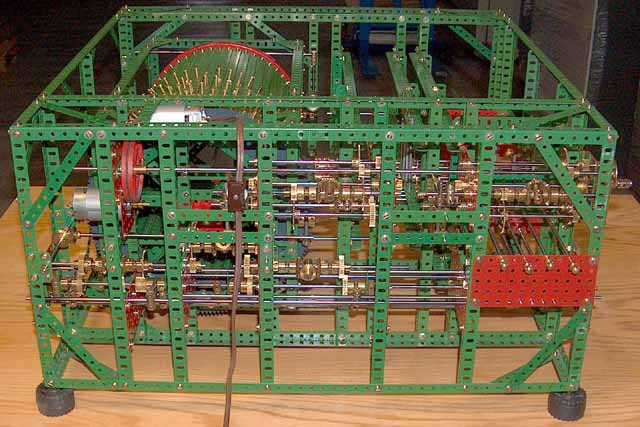
\includegraphics[width=0.3\textwidth]{imagens/babbage.jpg}
      
      % \end{figure}
      }
      } 
    % \raisebox{-\totalheight}{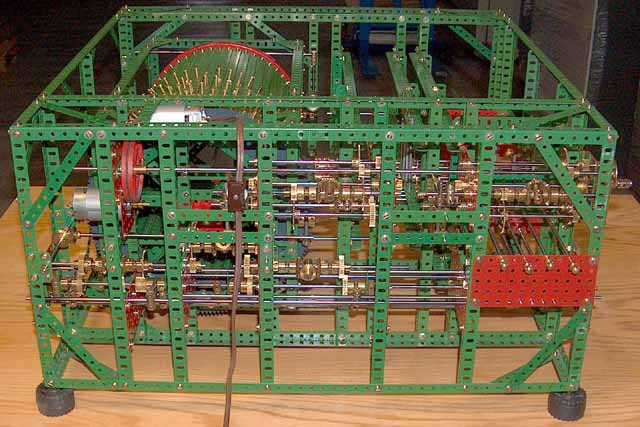
\includegraphics[width=0.3\textwidth, height=60mm]{imagens/babbage.jpg}}\\\\\cline{1-4}

    % \mutirow{4}{*}{
    % } \\ \cline{1-4}
  \end{tabular}